% "{'classe':('PSI'),'chapitre':'stat_mam','type':('cours'),'titre':'Rappels de Statique', 'source':'','comp':('B2-14'),'corrige':True}"
\setchapterimage{Header_Peugeot.jpg}
\setchapterpreamble[u]{\margintoc}
%\setcounter{chapter}{1}

\chapter{Rappels de Statique}

\marginnote[8cm]{
\xpComp{STAT}{02}
%\UPSTIcompetence[2]{B2-14}
%\UPSTIcompetence[2]{C2-03}
}



\section{Modélisation locale des actions mécaniques}
\begin{defi}[Action mécanique de contact volumique]
Localement, les actions mécaniques volumiques peuvent être modélisées par le torseur suivant :
$
\torseurstat{T}{1}{2}=
\torseurl{%
\vect{R_{(1\rightarrow 2)}} 
= \iiint\limits_{\mathcal{V}} f(M) \vect{u(M)} \text{d}\mathcal{V}}{%
\vectm{P}{1}{2} = \iiint\limits_{\mathcal{V}}\vect{PM}\wedge \text{d}\vectf{1}{2}}{M}
$.

La densité volumique d'effort s'exprime en $\left[\text{Nm}^{-3}\right]$.
\end{defi}

\begin{defi}[Action mécanique de contact surfacique]
Localement, les actions mécaniques dans un contact surfacique peuvent être modélisées par le torseur suivant :
$
\torseurstat{T}{1}{2}=
\torseurl{%
\vect{R_{(1\rightarrow 2)}} 
= \iint\limits_{\mathcal{S}} f(M) \vect{u(M)} \text{d}\mathcal{S}}{%
\vectm{P}{1}{2} = \iint\limits_{\mathcal{S}}\vect{PM}\wedge \text{d}\vectf{1}{2}}{M}
$.

La densité surfacique d'effort peut alors se décomposer sur le vecteur normal au contact et sur un vecteur appartenant au plan tangent au contact. On a alors$f(M) \vect{u(M)} = p_{12}(M)\vect{n_{12}}+\vect{\tau_{12}}(M)$. 
On note ;
\begin{itemize}
\item $p_{12}(M)$ pression de contact au point $M$ (en $\left[\text{Nm}^{-2}\right]$);
\item $\vect{\tau_{12}}(M)$ : la projection tangentielle de la densité surfacique (norme en $\left[\text{Nm}^{-2}\right]$).
\end{itemize}
\end{defi}

\section{Modélisation globale des actions mécaniques}

\begin{defi}[Torseur statique ou torseur sthénique ou torseur d'efforts]

L'action mécanique d'un système matériel $S_1$ (ou d'un phénomène physique) sur un système matériel $S_2$ est représentable par un torseur au point $M$:

$$
\torseurstat{T}{S_2}{S_1}
=\torseurl{\vectf{S_2}{S_1}}{\vectm{M}{S_2}{S_1}}{M}
=\torseurcol{X_{12}}{Y_{12}}{Z_{12}}{L_{12}}{M_{12}}{N_{12}}{M,\mathcal{R}}
$$
\end{defi}
\begin{remarque}
La norme de vecteur $\vectf{S_2}{S_1}$ est en Newton (N). La norme du vecteur $\vectm{M}{S_2}{S_1}$ est en Newton -- mètre ($N\cdot m$).
\end{remarque}

\begin{prop}[Varignon]
Le torseur statique étant un torseur, on a donc : 

$$
\forall B, \vectm{B}{S_2}{S_1} = \vectm{A}{S_2}{S_1} + \vect{BA} \wedge \vectf{S_2}{S_1}
$$
\end{prop}



\begin{marginfigure}
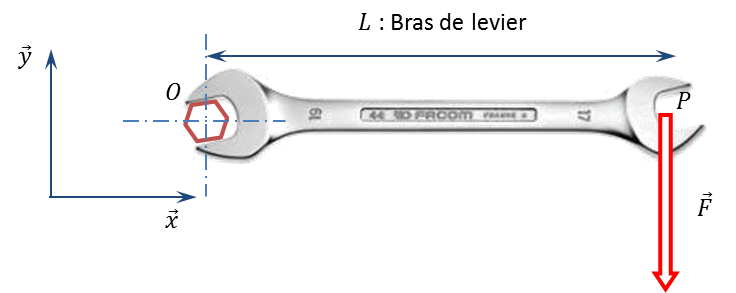
\includegraphics[width=\textwidth]{clef}
\end{marginfigure}

\begin{remarque}[\; -- Moment d'une force -- Interprétation graphique]

Prenons le cas du serrage d'un écrou avec un effort $\vect{F}=-F\vect{y}$ :


Dans l'hypothèse où l'effort $\vect{F}$ s'appliquerait au point $O$, il n'y aurait donc pas de serrage de l'écrou. Le moment (ou couple de serrage) serait donc nul : $\vectm{O}{\text{Clef}}{\text{Ecrou}}=\vect{0}$.

Si l'effort s'applique en $P$ :
$\vectm{O}{\text{Clef}}{\text{Ecrou}}=\vect{OP}\wedge\vect{F}
=L\vect{x}\wedge-F\vect{y}=-LF\vect{z}$.

Méthode pour déterminer le moment dans un problème plan : 
\begin{itemize}
\item norme du vecteur : effort fois bras de levier (on peut éventuellement décomposer l'effort dans le repère de travail);
\item perpendiculaire au plan;
\item sens : on regarde si, par rapport au point où on chercher le moment, l'effort fait tourner la pièce dans le sens direct ou indirect. 
\end{itemize}

\end{remarque}

\begin{figure}[!h]
\centering
\includegraphics[width=\linewidth]{pfs}
Application du TMS en $A$ : $C_B + Y_B L + 0 = 0$.
\end{figure}
